\documentclass[11pt,oneside]{book}

\usepackage[table]{xcolor}
\usepackage{titlesec}
\usepackage{mdframed}
\usepackage{wrapfig}

\usepackage{multirow}

\colorlet{rulercolor}{gray!50}
  
\titleformat{\chapter}
  {\normalfont\sffamily\Large\fontfamily{phv}\selectfont}
  {\thechapter.}{.5em}{}
  [\vspace{.2ex}\color{rulercolor}\titlerule]
  
\newmdenv[leftmargin=20pt, rightmargin=20pt, 
skipabove=\topsep,skipbelow=\topsep,
backgroundcolor=gray!30,shadow=true,shadowsize=4,
roundcorner=10pt]{shadebox}

\newmdenv[leftmargin=30pt, rightmargin=30pt, 
skipabove=0pt,skipbelow=0pt,
backgroundcolor=gray!10]{mybox}

\usepackage{graphicx}
%%	using final option to force graphics to be included even in draft mode
%\usepackage[final]{graphicx}
\usepackage{paralist} % compact lists

%% Support sub-figures.
\usepackage{subfigure}

%% Make subsections numbered and included in ToC
\setcounter{secnumdepth}{3}
\setcounter{tocdepth}{2}

%% Make margins less ridiculous
\usepackage[margin=1.15in]{geometry}

%% Package to linebreak URLs in a sane manner.
\usepackage{url}

%% Define a new 'smallurl' style for the package that will use a smaller font.
\makeatletter
\def\url@smallurlstyle{%
  \@ifundefined{selectfont}{\def\UrlFont{\sf}}{\def\UrlFont{\small\ttfamily}}}
\makeatother
%% Now actually use the newly defined style.
\urlstyle{smallurl}
%% Make URLs clickable
\usepackage[colorlinks, bookmarks=true]{hyperref}
\usepackage[all]{hypcap}


%% Since I'm using the LaTeX Makefile that uses dvips, I need this
%% package to make URLs break nicely
\usepackage{breakurl}

\usepackage{array}

%% Make table cross pages.
\usepackage{longtable}
\usepackage[table]{xcolor}

%% Make links to captions point to the figure, not just the caption at bottom
\usepackage[all]{hypcap}

% create a shortcut to typeset table headings
\newcommand\tabhead[1]{\small\textbf{#1}}

\graphicspath{{figures/}} 
\DeclareGraphicsExtensions{.eps}

\setlength{\headheight}{15.2pt}

\usepackage{fancyhdr}
\pagestyle{fancy}
	\renewcommand{\sectionmark}[1]{ \markright{#1}{} }
	\fancyhead[LE,RO]{\thepage}
	\fancyhead[RE]{\textit{ \nouppercase{\leftmark}} }
	\fancyhead[LO]{\textit{ \nouppercase{\rightmark}} }

\title{SGSEAM Assessment Guide for Lucid BuildingOS and BuildingDashboard}

\author{
	 Yongwen Xu \\
\em  Collaborative Software Development Laboratory \\
\em  Department of Information and Computer Sciences \\
\em  University of Hawai'i at Manoa\\
     yxu@hawaii.edu \\
}

\date{\today}

\begin{document}

\maketitle

\newpage

\tableofcontents
\newpage

\chapter{Introduction}
This document describes the proposed approach to assess the Lucid BuildingOS and BuildingDashboard using the Serious Game Stakeholder Experience Assessment Method (SGSEAM). The goal of SGSEAM assessment is to identify the major strengths and shortcomings of the framework from the perspectives of user experiences of major stakeholders. The benefits of this assessment are for the developers of the framework to learn from the findings of the assessment and identify any actionable improvements.
\newline

\autoref{fig:overview} outlines the steps of the process of applying SGSEAM to a framework.

\begin{figure}[ht!]
  \center
  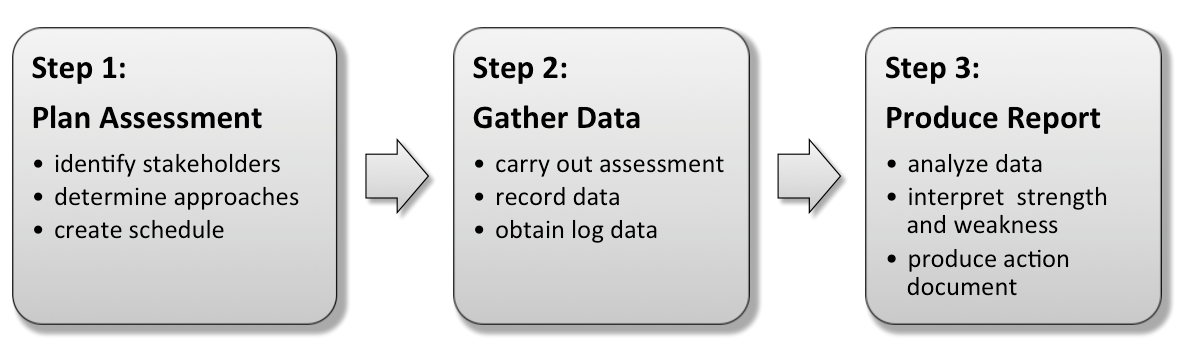
\includegraphics[width=0.8\columnwidth]{sgseam-steps}
  \caption{Applying SGSEAM to a framework}
  \label{fig:overview}
\end{figure}

There are three steps in the process of applying SGSEAM. Step one is to plan the assessment, including
 identifying the stakeholders, determine assessment approaches, and creating the assessment schedule. 
 The deliverable for this step is the \textbf{\textit{assessment plan}} document. Step two is to gather data by carrying out 
 the assessment, record and obtain any related data. The deliverable for this step is the 
 assessment \textbf{\textit{data repository}}. Step three is to produce the strength and weakness report by analyzing 
 the data and interpreting strengths and weaknesses. The deliverable for this step is the \textbf{\textit{improvement action}} document.
 \newline

 The following chapters describe the steps in details.

\chapter{Plan Assessment}

\section{Identify Stakeholders}

\begin{shadebox}
\begin{wrapfigure}{l}{0.04\textwidth}
\vspace{-15pt}\hspace{-10pt}
    
\includegraphics[width=0.04\textwidth]{note-icon}
\end{wrapfigure}

Identify the stakeholders in each SGSEAM stakeholder class, write down their names and contact info.

\end{shadebox}

The first step of SGSEAM assessment is to identify stakeholders of the framework. For Lucid BuildingOS and BuildingDashboard, We will select a few organizations who participated in the Campus Conservation National (CCN) 2014 and used BuildingOS and BuildingDashboard framework to create their competitions. From these organization, we will identify the persons by their stakeholder roles as defined in \autoref{table:stakeholders}. 

\begin{table}[ht!]
  \centering
  \begin{tabular}{|p{0.2\columnwidth}|p{0.4\columnwidth}|p{0.3\columnwidth}|}
    \hline
    \tabhead{Stakeholder class} &
    \tabhead{Definition} &
    \tabhead{Person(s)} \\
    \hline
    Players &
    Residents living in the buildings that participate in the competition. &
    emails \\
    \hline
    System admins &
    IT staffs who are responsible for setting up and maintain the software infrastructure for the competition. &
    name, contact \\
    \hline
    Game designer &
    Competition organizers who design and configure the competition such as content experts, designers. &
    name, contact \\
    \hline
    Game managers &
    Competition organizers who is responsible for running the competition such as residential life staff, sustainability coordinator&
    name, contact\\
    \hline
    Game developers &
    Software developers who use the framework to customize, extend and enhance the game. &
    name, contact \\
    \hline
  \end{tabular}
  \caption{SGSEAM Stakeholders}
  \label{table:stakeholders}
\end{table}

For each stakeholder, identify the population, the name and contact info. It is important to be able to contact the stakeholders in some way, either via email or phone, to get the feedback from their experiences with 
the framework.
\newline
\newline

\section{Determine Assessment Approach}
\label{sect:Assessment Approach}

\begin{shadebox}
\begin{wrapfigure}{l}{0.04\textwidth}
\vspace{-15pt}\hspace{-10pt}
    
\includegraphics[width=0.04\textwidth]{note-icon}
\end{wrapfigure}
For each stakeholder, determine the appropriate assessment approaches.
\end{shadebox}

There are several assessment approach for each stakeholders. Different assessment approaches have different levels of rigor which represents confident level of the assessment result. Different approaches also require different levels of implementation costs or efforts. Due to the efforts in recruiting testing subjects and set up the experiments, in-lab experiment assessment may be too expensive in the case of assessing BuildingOS and BuildingDashboard. \autoref{table:approaches} shows the recommended assessment approaches for the stakeholders in BuildingOS and BuildingDashboard. The following sections describes the details for the approaches.
 
\begin{table}[ht!]
  \centering
  \begin{tabular}{|p{0.175\columnwidth}|p{0.28\columnwidth}|p{0.42\columnwidth}|}
    \hline
    \tabhead{Stakeholder}&
    \tabhead{Assessment approaches}&
    \tabhead{Expected outcomes } \\
    \hline
    \multirow{3}{*}{Player}&
    	Pre-post effectiveness study (\ref{Pre-Post effectiveness study}) &
	Determine effectiveness in resource usage reduction.\\\cline{2-3}
        &
	Self-reported usability metrics (\ref{Self-reported usability metrics}) &
	identify problem areas in game interface\\\cline{2-3}
        &
	Engagement metrics (\ref{Engagement metrics}) &
	determine the extent of engagement\\
    \hline
    System admin&
    	Post-hoc admin interview (\ref{Post-hoc system admin interview}) &
	identify strengths and weaknesses in the installation and maintenance process.\\
    \hline
    Game designer&
    	Post-hoc designer interview (\ref{Post-hoc game designer interview}) &
	Determine strengths and weaknesses in the game design interface.\\
    \hline
    Game manager&
    	Post-hoc manager interview (\ref{Post-hoc game manager interview}) &
	Determine strengths and weaknesses in the game managing interface.\\
    \hline
    Game developer&
    	Post-hoc developer interview (\ref{Post-hoc game developer interview}) &
	Determine strengths and weaknesses in developing enhancement.\\
    \hline
  \end{tabular}
  \caption{Lucid SGSEAM Assessment Approaches}
  \label{table:approaches}
\end{table}
      
\subsection{Player Assessment}

The goal of player assessment is to determine the effectiveness of the game
framework from player's perspective as well as the usability of the game interface and the engagement level of the game. 
We proposes three approaches for assessing the player's experience with Lucid's framework.

\subsubsection{Player Assessment Approach: Pre-post Effectiveness Study}
\label{Pre-Post effectiveness study}

One of the goals of the competition is (but not limited to) the reduction of resource such as energy and water consumption. To assess the effectiveness of this goal, we need to determine the metrics that may be measured before and after the competition (pre-post). Lucid BuildingOS and Dashboard calculates the percentage of reduction of energy and water consumption for each participated building, based on the baseline usage of the previous two weeks. We will use this metrics to measure the effect of the competition. The maximum, minimum and average percentage of reduction of all the buildings are calculated to determine the most, the least and average reduction of the resource usage. 

This assessment reveals the extend of effectiveness of the game produced by the framework, regarding to the resource consumption reduction. 
  
\subsubsection{Player Assessment Approach: Self-reported Usability Metrics} 
\label{Self-reported usability metrics}

We will conduct a player usability survey at the final week or right after the competition to understand the strengths and weaknesses of the game user interface perceived by players. Minimum of 20 players (the more the better) are randomly selected to participate in this survey. The survey is administrated online via survey monkey or other survey tools. We design the survey questionnaire as shown in \autoref{fig:usability-metrics}.
       
\begin{figure}[ht!]
\begin{mybox}
\begin{compactenum}
\item What did you like most about the game?
\item What did you found confusing?
\item What issues did you have while using the game?
\item What was the thing you liked the least about the game?
\item What can we do to improve the game?
\item It was easy to find what I was looking for on the website.  \\
	Strongly disagree  -  Disagree  -  Neutral  -  Agree  -  Strongly agree
\item The website was responsive. \\
	Strongly disagree  -  Disagree  -  Neutral  -  Agree  -  Strongly agree
\item The website provided adequate help in teaching me how to play. \\
	Strongly disagree  -  Disagree  -  Neutral  -  Agree  -  Strongly agree
\item I understood how to play. \\
	Strongly disagree  -  Disagree  -  Neutral  -  Agree  -  Strongly agree
\item this is something my friends should participate in. \\
	Strongly disagree  -  Disagree  -  Neutral  -  Agree  -  Strongly agree
\end{compactenum}
\end{mybox}
\caption{Player self-reported usability metrics questionnaires}
\label{fig:usability-metrics}  
\end{figure}

Once the survey is created online, the survey administrator will email the selected players with the link and instruction to the online survey. 
After we received all the survey responses, we will code and analyze the response to understand the areas of usability problems in the game interface as well as the areas of strengths.

This assessment reveals the strengths and weaknesses of the framework regarding the usability of the game interface.
 
\subsubsection{Player Assessment Approach: Engagement Metrics}
\label{Engagement metrics}

This approach calculates the engagement metrics to assess the extent of engagement from players and the impact of the game. The more engaging the game is, the more potential impact could be to the players.

We will first obtain the detailed logs of user interaction with the game. These logging includes http web server logs and user action logs which identify every user click on the web page. Once the log data are available, we will calculate the engagement metrics as described in \autoref{figure:engagement-metrics}. Calculate as many as possible the player engagement metrics. The more metrics obtained, the better understanding of the extent of player engagement.

\begin{figure}[ht!]
  \centering
    \begin{tabular}{|p{0.2\columnwidth}|p{0.28\columnwidth}|p{0.32\columnwidth}|}
    \hline
    \tabhead{Metric} &
    \tabhead{Definition} &
    \tabhead{Mesure} \\
    \hline
    participation &
    percentage of players who play the game &
    the level of involvement from players \\
    \hline
    player &
    number of players per day &
    the frequency of players interact with the game \\
    \hline
    play time &
    play time of a player per day &
    the frequency of players interact with the game \\
    \hline
    submission &
    submissions of all player per day &
    the rate of players' completion of game activities \\
    \hline
    social interaction &
    social interaction of all player per day &
    the rate of in-game social interactions between players\\
    \hline
    game error &
    game errors per day &
    the rate of errors encountered by players during the game \\
    \hline
  \end{tabular}
  \caption{Player engagement metrics}
  \label{figure:engagement-metrics}
\end{figure}

With the exception of the game error metric, the higher value these metrics are, the higher engagement level the game has. 
Distribution of the above metrics across of the period of the competition also provides insights on 
the extent of engagement in different time of the competition. For example, it may be typical that
the first few days of the competition may have higher number of player and play time metrics because 
of the launch, or due to the announcement of an interesting real-world event. 

This assessment reveals the extent of engagement of the players in the game.

\subsection{System Admin Assessment}

The goal of system admin assessment is to determine to what extent the 
framework facilitates the system administration tasks from system admin's perspective. SGSEAM 
assesses how much time is required to install and maintain an instance of a serious game using the 
framework and the problems encountered  during the system admin process.

We consider the tasks of system admin interacting with Lucid's framework are:
\begin{compactenum}
    \item install the software
    \item configure smart meter connectivity
    \item backup data
    \item monitor performance
    \item scaling the system
    \item patching
\end{compactenum}

We propose the post-hoc system admin interview approach to assess the system admin's experience for Lucid's framework.

\subsubsection{System Admin Assessment Approach: Post-loc System Admin Interview}
\label{Post-hoc system admin interview}

Once we identify the contact information of the system admins, the interview will be administrated by using an online questionnaire form followed by an optional phone interview if needed. We design the interview with the following questionnaire that is tailored to the specific tasks of the system admins of Lucid's framework:

\begin{figure}[ht!]
\begin{mybox}
\begin{compactenum}
\item How much time did you spend to install the system and the dependencies?
\item How much time did you spend to configure the meters?
\item How much time did you spend to maintain the system such as backup, patching, monitoring?
\item Did you need to scale the system? if Yes, how much time did you spend?
\item What problems did you encounter?
\item Did you find it difficult to admin the system? What was difficult?
\item Do you agree for us to call you for a short phone interview if we have more questions regarding your experience with the system?
\end{compactenum}
\end{mybox}
\caption{System admin interview questionnaires}
\label{fig:system-admin-interview}  
\end{figure}

Once we receive the responses from the system admin, we will code (categorize) the time and problems encountered to find out what are the problem areas if there is any. if we need further explanation to the response, we will administrate a quick phone interview to address the specific response. 

These assessment reveals the strengths, weaknesses and the areas of improvement regarding the system admin process for the framework.

\subsection{Game Designer Assessment}

The goal of SGSEAM game designer assessment is to determine the strengths and weaknesses of the framework 
regarding to the game design process. SGSEAM 
assesses how much time is required to design an instance of a serious game using the framework and the problems encountered during the design process.

We consider the tasks of game designer interacting with Lucid's framework are:
\begin{compactenum}
    \item decide competition period
    \item set up building occupancy, manual or automated meters
    \item decide baseline period
    \item monitor competition status during the competition
\end{compactenum}

We propose the post-hoc game designer interview approach to assess the game designer's experience.

\subsubsection{Game Designer Assessment Approach: Post-hoc Game Designer Interview}
\label{Post-hoc game designer interview}

 The interview is administrated by using an online questionnaire form followed by an optional phone interview if needed. We will interview several game designers of different competitions. The more data we collect, the more insights we get. The interview is designed with the following questionnaire that is tailored to the specific tasks of the game designers of Lucid's framework:

\begin{figure}[ht!]
\begin{mybox}
\begin{compactenum}
\item How much time did you spend to set up the buildings including meters?
\item How much time did you spend to setup the competition (competition periods, baseline period, participants)?
\item How much time did you spend to setup the homepage by deciding which widgets to include?
\item How much time did you spend to monitor analytical data to understand the state of the game
\item What problems did you encounter?
\item Did you find it difficult to use the interface? What was difficult?
\item Do you agree for us to call you for a short phone interview if we have more questions regarding your experience with the system?
\end{compactenum}
\end{mybox}
\caption{Game designer interview questionnaires}
\label{fig:game-designer-interview}  
\end{figure}

After the interview, code and categorize the reported time and problems to identify the strengths and weaknesses. In addition, if possible, collect the system log data related to the game designing tasks, analyze the logs to find out the time spent and error encountered during the game designing tasks. Use the log data to verify the findings from the interview data.

These assessment reveals the strengths, weaknesses and the areas of improvement regarding the game design process for the framework.

\subsection{Game Manager Assessment}

The goal of SGSEAM game manager assessment is to determine the strengths and weakness of the framework 
regarding to the game management process. Similar to the assessment of the game designer, SGSEAM assesses 
how much time it is required to manage an instance of a serious game using the framework
and the problems encountered during the managing process.

We consider the tasks of game manager interacting with Lucid's framework are:
\begin{compactenum}
    \item input data manually
    \item manage events, marketing, handing out prizes
    \item monitor competition status
\end{compactenum}

we propose the post-hoc game manager interview approach for assessing game manager's experience.
    
\subsubsection{Game Manager Assessment Approach: Post-hoc Game Manager Interview}
\label{Post-hoc game manager interview}

 The interview is administrated by using an online questionnaire form followed by an optional phone interview if needed. We will interview several game managers of different competitions. The more data we collect, the more insights we get.  The interview is designed with the following questionnaire that is tailored to the specific tasks of the game managers of Lucid's framework:

\begin{figure}[ht!]
\begin{mybox}
\begin{compactenum}
\item How much time did you spend to enter the meter data manually for the baseline period?
\item How much time did you spend to enter the meter data manually for the competition period?    
\item What problems did you encounter?
\item How much time did you spend to monitor analytical data to understand the state of the game
\item Did you find it difficult to manage? What was difficult?
\end{compactenum}
\end{mybox}
\caption{Game manager interview questionnaires}
\label{fig:game-manager-interview}  
\end{figure}

After the interview, code and categorize the reported time and problems to identify the strengths and weaknesses in the game managing process. In addition, if possible, collect the system log data related to the game managing tasks, analyze the logs to find out the time spent and error encountered during the game managing tasks. Use the log data to verify the findings from the interview data.

These assessment reveals the strengths, weaknesses and the areas of improvement regarding the game managing process for the framework.

\subsection{Game Developer Assessment}

To investigate how easy it is to understand, extend, and debug a serious game framework from a developer's 
perspective, SGSEAM assesses how much time it takes to develop an
enhancement to the game framework, and how many errors are encountered
during the development process.

We consider the tasks of game manager interacting with Lucid's framework are:

\begin{compactenum}
  \item use API to get data in and/or out of the system
  \item customize the interface
  \item extend the system to support new meters
  \item enhancement
\end{compactenum}

We propose the post-hoc game developer interview approach to assess the game developer's experience.
    
\subsubsection{Game Developer Assessment Approach: Post-hoc Game Developer Interview}
\label{Post-hoc game developer interview}

BuildingOS and Dashboard have APIs for developing apps to tie into the framework. We will use the API to develop an extension or customization of the system. Here are the development tasks we proposed to perform using Lucid's API to extend the framework:
\begin{compactenum}
  \item create a new widget to be available in the home page.
  \item support the automated energy data collection from a new type of meter.
\end{compactenum}

We will ask the identified game developers to perform the above development tasks using Lucid's framework. The developer could be Lucid internal developers or some one outside of Lucid.  After the development tasks are completed, we will interview the developers to assess his experience for these development tasks. The interview is designed with the questionnaire outlined in \autoref{fig:game-developer-interview}.

\begin{figure}[ht!]
\begin{mybox}
\begin{compactenum}
\item How much time did you spend to implement the creation of a new widget?
\item How much time did you spend to implement adding a new type of meter?
\item What problem(s) did you encounter?
\item Did you find it difficult to understand, extend and debug the system? What was difficult?
\end{compactenum}
\end{mybox}
\caption{Game developer interview questionnaires}
\label{fig:game-developer-interview}  
\end{figure}

Once the interview data is collected, categorize the reported problems and correlated with the reported time data to identify the areas of strength (less time spent) and weakness (more time spent and problems or difficulties) in the process of development. 

These assessment reveals the strengths, weaknesses and the areas of improvement regarding the game development process for the framework.

\section{Create Assessment Plan}
\begin{shadebox}
\begin{wrapfigure}{l}{0.04\textwidth}
\vspace{-15pt}\hspace{-10pt}
    
\includegraphics[width=0.04\textwidth]{note-icon}
\end{wrapfigure}
Create a schedule for each assessment, produce the assessment plan document.
\end{shadebox}

Once we decide what the assessment approaches and who the participants are, the next step is to create the assessment 
schedule and produce the assessment plan document. The document should include the detailed assessment plan for 
each stakeholder class. 

\autoref{figure:assessment-plan} shows an example of the assessment schedule broken down in the tasks 
in the plan document.

\begin{figure}[ht!]
  \centering
  \begin{tabular}{|p{0.5\columnwidth}|p{0.15\columnwidth}|p{0.15\columnwidth}|}
    \hline
    \multicolumn{3}{|c|}{\tabhead{Game design assessment approach: post-hoc game designer interview}} \\
    \hline
    \tabhead{Task} &
    \tabhead{Estimated Start date} &
    \tabhead{Estimated End date} \\
    \hline
    Design the interview questionnaire & & \\
    \hline
    send out the questionnaires to the game designer(s) & & \\
    \hline
    Collect response data from participants & & \\
    \hline
    Obtain log data & & \\
    \hline
    Analyze the data & & \\
    \hline
    Interpret strength and weakness & & \\
    \hline
    Produce action document & & \\
    \hline
  \end{tabular}
  \caption{Assessment schedule in the plan document}
  \label{figure:assessment-plan}
\end{figure}


\chapter{Gather Data}
This step carries out the assessment, record the data, obtain log data, and refine the assessment plan if necessary. 
The output of this step is a data repository contains all the assessment data that can be analyzed in the next step.

\section{Carry Out Assessment}
\begin{shadebox}
\begin{wrapfigure}{l}{0.04\textwidth}
\vspace{-15pt}\hspace{-10pt}
    
\includegraphics[width=0.04\textwidth]{note-icon}
\end{wrapfigure}
Carry out the assessment as described in the assessment plan.
\end{shadebox}

For each assessment approach, complete the tasks outlined in the assessment plan, gather the data when carrying out the 
assessment. Store all the data into a central data repository. 

\section{Obtain Log Data}
\begin{shadebox}
\begin{wrapfigure}{l}{0.04\textwidth}
\vspace{-15pt}\hspace{-10pt}
    
\includegraphics[width=0.04\textwidth]{note-icon}
\end{wrapfigure}
Obtain the log data from the framework, including all the interaction log from the each stakeholder.
\end{shadebox}

Talk to the technical staffs of the framework to find out what kind of log data is available. Obtain the log data in a format that 
is easy to analyze. For example, if the log data is in a database table, ask for the access to the table, or the CSV export of 
the table data. If the log data is in a log file, ask for the access to the file. Store the log data into the central data repository.

\chapter{Produce Strength and Weakness Report}

This step analyzes all the data gathered from previous steps, interpret the strengths and weakness of the framework, 
and produce the action report regarding to what areas of the framework needs to improve on.

\section{Analyze Data}
\begin{shadebox}
\begin{wrapfigure}{l}{0.04\textwidth}
\vspace{-15pt}\hspace{-10pt}
    
\includegraphics[width=0.04\textwidth]{note-icon}
\end{wrapfigure}
Analyze the data from the data repository.
\end{shadebox}

This step performs the data analysis from the data repository obtained from the previous step. Follow the assessment approaches described in \autoref{sect:Assessment Approach} for each stakeholder to carry out the data analysis. For example, for player assessment, calculate the 
engagement metrics from the game log; for game designer assessment, perform queries from user interaction log data to find out the completion time for a certain game designing task such as completing the configuration of global game settings. 

\section{Interpret Strength and Weakness}
\begin{shadebox}
\begin{wrapfigure}{l}{0.04\textwidth}
\vspace{-15pt}\hspace{-10pt}
    
\includegraphics[width=0.04\textwidth]{note-icon}
\end{wrapfigure}
Interpret strengths and weaknesses of framework from the data analysis.
\end{shadebox}

From the data analysis step, identified the problem areas which are indicated by having the most reported problems and the 
longest completion time. 

\section{Produce Reports with Actionable Steps}
\begin{shadebox}
\begin{wrapfigure}{l}{0.04\textwidth}
\vspace{-15pt}\hspace{-10pt}
    
\includegraphics[width=0.04\textwidth]{note-icon}
\end{wrapfigure}
Produce the action reports for any improvement identified from the strength and weakness analysis.
\end{shadebox}

Once the strength and weakness of the framework are identified from the data analysis, an action report should be produced. 
This report includes the weakness areas that can be improved and actionable steps on how to improve from 
each stakeholder's perspective. It also includes the strength areas that the framework needs to maintain.

By producing the report with actionable steps to improve the framework, the SGSEAM assessment is completed.  

%% Use this for an alphabetically organized bibliography
\bibliography{sustainability,csdl-trs,gamification,yxu}
\bibliographystyle{plain}

\end{document}
